\section{SPI Driver in Julia Programming Language}

The github project from which mine was derived uses a programming language called ``Julia'' in the JTAG server and for image data processing:

\url{https://julialang.org/}

This was a language I had heard about, but I had never tried it.
To duplicate and run the original project, I had to install the language binary.
The program does the processing of the GIF image, and then sends the data to the FPGA
via the JTAG server and USB-to-JTAG interface.

It was simple to install the server and run the Julia program.  It all worked first time!
Later, I installed the Atom IDE which has a Julia plug-in.  It's great!

Rather than reinventing the wheel, I decided to use the image processing portion of the Julia program.
However, how to drive the FTDI SPI device?  I needed something to replace the JTAG server.

The FTDI USB-to-SPI device is supported with a C shared library.  This library has the initialization, read, write, and shutdown
command necessary to work with the device.

Fortuitously, the Julia language includes the capability to call C library functions in a very direct way!
I was skeptical at first, but I quickly had the SPI device's initialization function running and returning with no error.
The other required functions were quickly added.  I now had full control of the SPI bus from the command line!

When I say ``command line'', in the case of Julia I am referring to the ``Read Eval Print Loop'', called the REPL.  This functionality is similar to Python, and is my favorite way to develop code.  I also used the ``Atom'' IDE, which has a plug-in for the Julia language.
It is a new language, and has a few quirks like all of them do, but so far I am impressed!

At first, Julia was also used to access a shared library which was taken from an Altera demo project of the SPI-Avalon bus master.
This library was responsible for reading and writing ``Avalon Packets''.  This is the protocol used by the Avalon bus.  I was able to successfully translate the Altera library to Julia.  This is working well and the system is able to read and write to the SPI and thus the FPGA Avalon bus, the parallel ports, and the SDRAM.

\begin{figure}[ht]
	\centering
	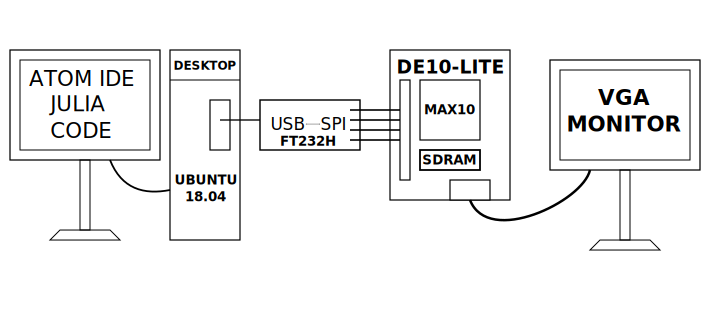
\includegraphics[width=0.7\textwidth]{images/project_system}
	\centering\bfseries
	\caption{Project System:  Desktop -> USB-to-SPI -> FPGA -> VGA Monitor}
\end{figure}

The Julia code is located in the ``src'' directory of the github repository linked in the introduction.
